\documentclass[12pt,landscape,twocolumn]{article}

%\input{art/cozydefs.tex}
\usepackage{productnote}

\usepackage{epsfig}
\usepackage{bookman}

\setlength{\oddsidemargin}{0in}		% default=0in
\setlength{\textwidth}{9in}		% default=9in

\setlength{\columnsep}{0.5in}		% default=10pt
\setlength{\columnseprule}{0pt}		% default=0pt (no line)

\setlength{\textheight}{6.5in}		% default=5.15in
\setlength{\topmargin}{-0.45in}		% default=0.20in
\setlength{\headsep}{0in}		% default=0.35in

\pagestyle{empty}	%no page numbers

\begin{document}

\section*{{\tt cozybit} Zeroconf module}
The cozybit Zeroconf module allows devices to advertise services and announce 
themselves to users without requiring extensive network configuration.  With 
Zeroconf, an embedded system can:

\begin{itemize}
	\item Quickly point users to its web-based configuration page.
	\item Announce a wireless VOIP handset on the network.
	\item Enable users to browse for services such as printers, media
		  devices, and network-attached storage.
\end{itemize}

\vspace{0.5in}
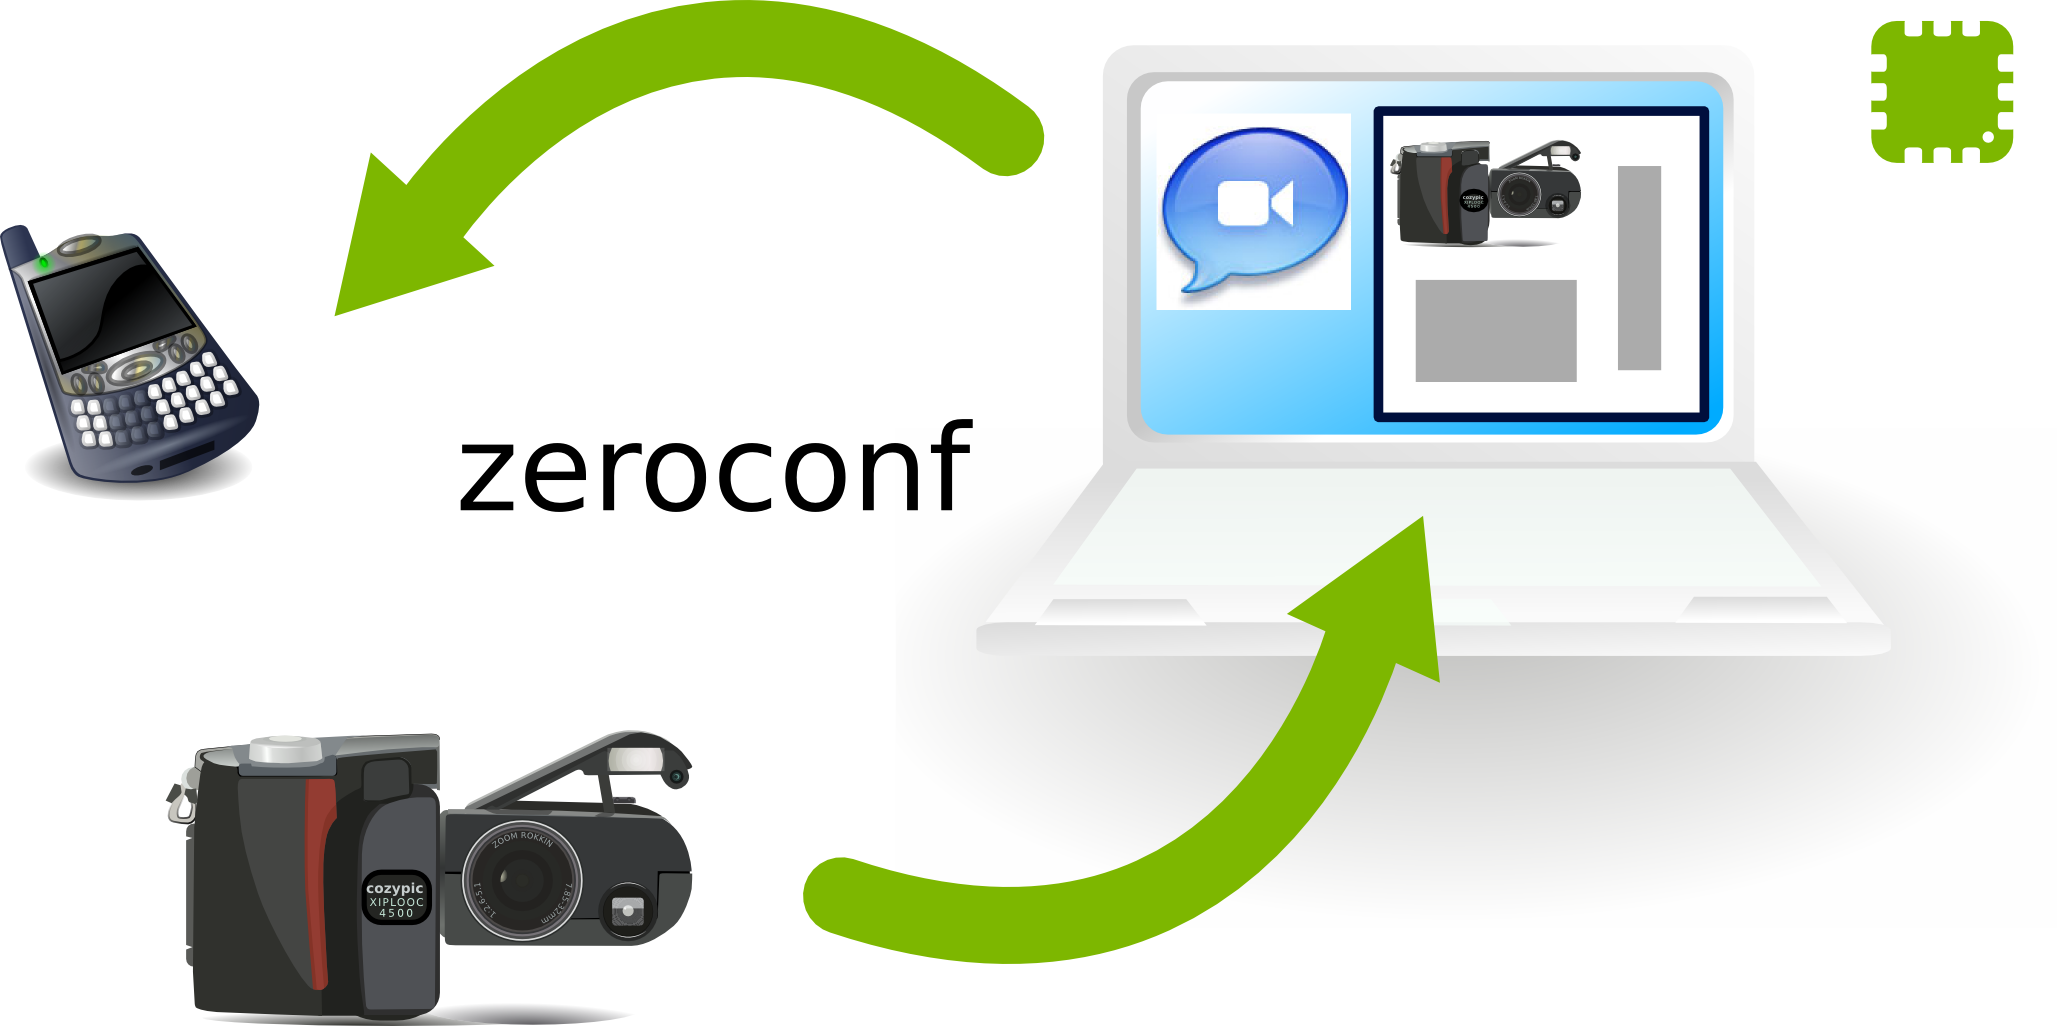
\includegraphics[width=4.5in]{zeroconf.png}
\vspace{0.5in}

\subsection*{Features}

The cozybit Zeroconf module provides:

\begin{itemize}
	\item Multicast DNS (mDNS) for automatic name resolution without the
		  presence of a DNS server.
	\item mDNS Responder, enabling the device to advertise its services on
		  to DNS-SD (Service Discovery) browsers on the network.
	\item mDNS Responder API, allowing the developer to configure the device
		  to advertise a desired name and service or services.
	\item IP4LL (Link Local) address self-assignment when it is needed.
	\item Adherence to current Zeroconf and mDNS draft standards and 
		  compatibility with Zeroconf implementations on Apple, Windows, and
		  Linux PCs.
	\item OS and TCP/IP stack independence.
\end{itemize}


\subsection*{Details}

The cozybit Zeroconf module is designed for small embedded systems.  The mDNS 
Responder runs in a single thread and does not require the use of dynamically 
allocated memory.  The mDNS service, at multicast address 224.0.0.251, uses 
UDP port 5353.

IP4LL allows devices to self-assign IP addresses in the 169.254/16 prefix. 
This allows devices to communicate on networks without DHCP or user 
configuration and is especially useful in ad-hock wireless networks.  The mDNS
Responder is capable of using an assigned IP or an IP4LL-provided address when
needed.

The module consists of an mDNS Responder thread and an optional IP4LL thread 
for Link Local address self-assignment.  An OS abstraction layer allows the 
module to be easily ported to many platforms.

\begin{center}
%\psfig{figure=./figures/arch.eps,angle=0,width=40ex}
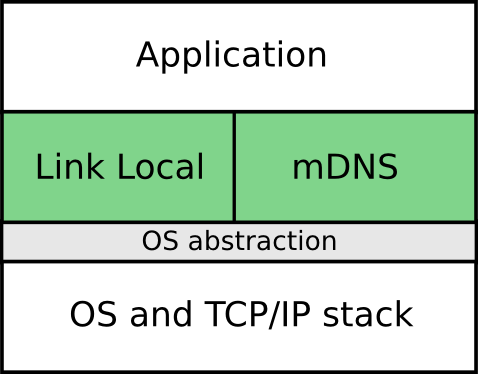
\includegraphics[width=40ex]{./figures/arch.png}
\end{center}

\subsection*{Supported Platforms}

At this time, the cozybit Zeroconf module has been ported to Linux and
Marvell 8388V ({\tt nohost SDK}).  The module's footprint when compiled with
the ARM ADS toolchain is approximately 8KB.

\pagebreak
\subsection*{Standards}

Please refer to the following draft standards and RFCs for details about the
Zeroconf draft standard:

\vspace{1ex}
\begin{tabular}{|l|l|}
\hline
mDNS & draft-cheshire-dnsext-multicastdns \\
\hline
DNS-SD & draft-cheshire-dnsext-dns-sd \\
\hline
DNS SRV & rfc2782 \\
\hline
IPV4LL & rfc3927 \\
\hline
\end{tabular}

\subsection*{Contact}
For additional product information please contact Javier Cardona at the numbers
printed below.

\strut{\vspace{1in}}
\begin{center}
\includegraphics*{art/cozybit-logo.pdf}\\
\vspace{3ex}
{\scriptsize 
\begin{tabular}{l l}
Tel: +1 415 974 6770   & 165 Jessie St. \\
Fax: +1 415 974 6771    & San Francisco, CA 94105 \\
http://www.cozybit.com  & USA \\
\end{tabular}}
\end{center}

\end{document}
